\documentclass[]{article}
\usepackage{graphicx}

%opening
\title{Summary of Hall C Spectrometer surveys}
\begin{document}
%	\maketitle
\section{HMS Surveys}
	Summary of HMS surveys done mostly during the summer of 2017. Define the pointing in the spectrometer coordinate system with +X downwards and +Y towards smaller angles.
		Table~\ref{tab:hms} lists measured mispointing in horizontal and vertical for each survey number and HMS angle. The horizontal mispointing is plotted versus HMS angle in Fig~\ref{fig:hms_horz_pointing} and shows a definite trend with angle. This was see before in the 6~GeV era. Survey at 60 and 70$^{\circ}$ would be useful to map out the dependence at above 40 degrees, since the 50 degree point indicates that the horizontal mispointing is changing. The vertical mispointing is plotted versus
		HMS angle in Fig~\ref{fig:hms_vert_pointing} and indicates a slight dependence on
		angle.
	
	\begin{table}[h]
	\begin{center}
	\begin{tabular}[]{|c|c||c|c|} \hline\hline
		Survey & HMS Angle  & Horizontal point (Y$_{spec}$) & Vertical point (X$_{spec}$)\\ \hline
		C1876  & 65.00  & +3.32 & +1.22 \\ \hline
		C1809R & 50.00  & +2.92 & +1.07 \\ \hline
		C1792R & 40.534 & +3.45& +0.91\\ \hline
		C1807R & 40.013 & +3.29 & +0.94 \\ \hline
		C1842 & 35.944 & +2.67 & +0.82\\ \hline
		C1842  & 25.013 & +1.47 &  +0.92 \\ \hline
		C1842  & 15.004 & +0.76 & 1.29\\ \hline
			C1842  & 15.005 & +0.82 & 1.45 \\ \hline
	\end{tabular}
	\caption{Table of HMS surveys}
	\label{tab:hms}
				\end{center}
	\end{table}


\section{SHMS Surveys}
Define the pointing in the spectrometer coordinate system with +X downwards and +Y towards larger angles.
Table~\ref{tab:shms} lists measured mispointing in horizontal and vertical for each survey number and SHMS angle. The horizontal mispointing is plotted versus SHMS angle in Fig~\ref{fig:shms_horz_pointing}.  The vertical mispointing is plotted versus
SHMS angle in Fig~\ref{fig:shms_vert_pointing}. 
			
			 	\begin{table}[h]
				\begin{center}
						\begin{tabular}[]{|c|c||c|c|} \hline\hline
		Survey & Angle  & Horizontal point (Y$_{spec}$) & Vertical point (X$_{spec}$)\\ \hline
        C1793  & 7.4787 & +0.06 & -1.29 \\ \hline
		C1876  & 10.00 & -1.48& -0.13\\ \hline
		C1812  & 15.01  & -0.74 & -1.34 \\ \hline
		C1806R & 15.02 & -0.38 & -1.16 \\ \hline
		C1876  & 20.00 & -0.60& +0.13\\ \hline
		C1796R & 20.32 & -0.57& -0.27\\ \hline
		C1808R & 24.99  & -0.43 & -1.28 \\ \hline
	    C1790  & 24.61 & -.87   &  -0.21 \\ \hline
		C1810R & 39.94  & -0.43 & -1.25 \\ \hline
		 		 	\end{tabular}
	\caption{Table of SHMS surveys}
	\label{tab:shms}
				\end{center}
				
	
		\end{table}
		\begin{figure}[h]	
			\begin{center}
				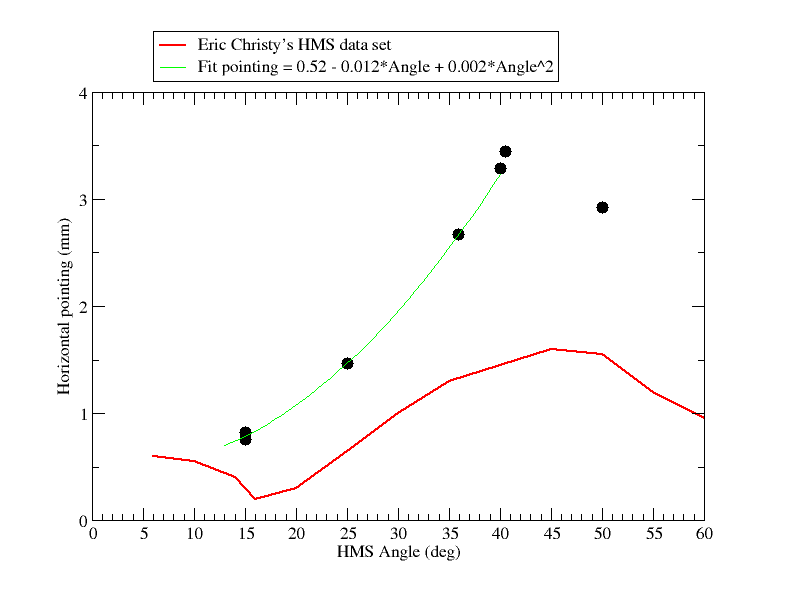
\includegraphics[width=0.8\columnwidth]{hms_horizontal_pointing.png}
			\end{center}
			\caption{HMS horizontal pointing versus HMS angle. The fit is to the data points at 35 degrees and below. }
			\label{fig:hms_horz_pointing}
		\end{figure}
		
		\begin{figure}[h]	
			\begin{center}
				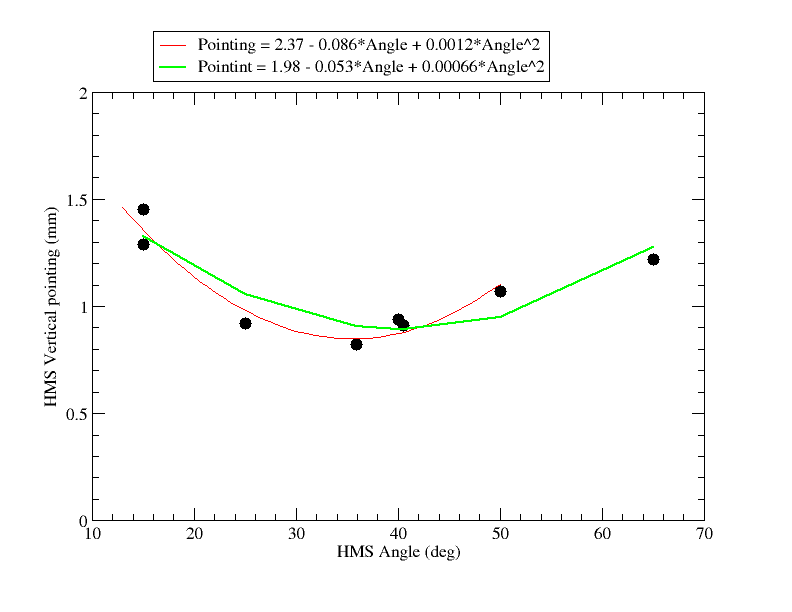
\includegraphics[width=0.8\columnwidth]{hms_vertical_pointing.png}
			\end{center}
			\caption{HMS vertical pointing versus HMS angle. The fit is to all the data points. }
			\label{fig:hms_vert_pointing}
		\end{figure}
		
		\begin{figure}[h]	
			\begin{center}
				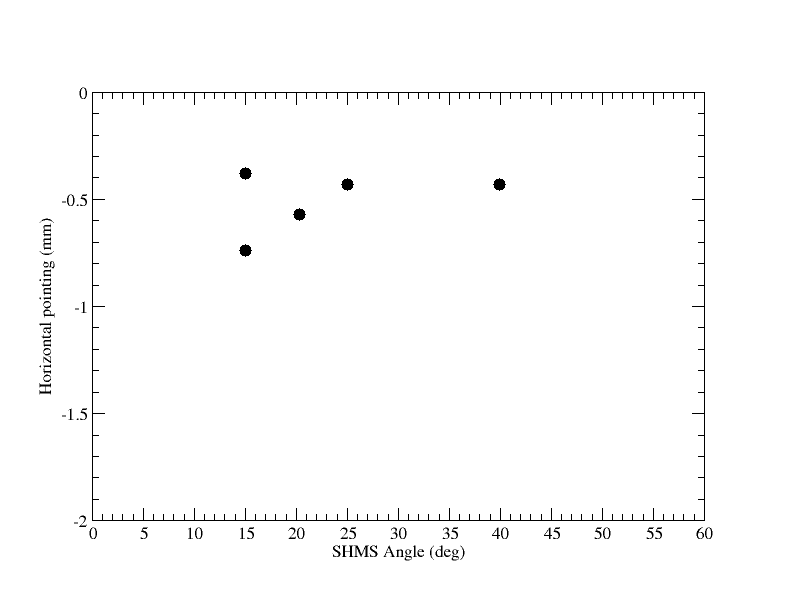
\includegraphics[width=0.8\columnwidth]{shms_horizontal_pointing.png}
			\end{center}
			\caption{SHMS horizontal pointing versus SHMS angle.  }
			\label{fig:shms_horz_pointing}
		\end{figure}
		
		\begin{figure}[h]	
			\begin{center}
				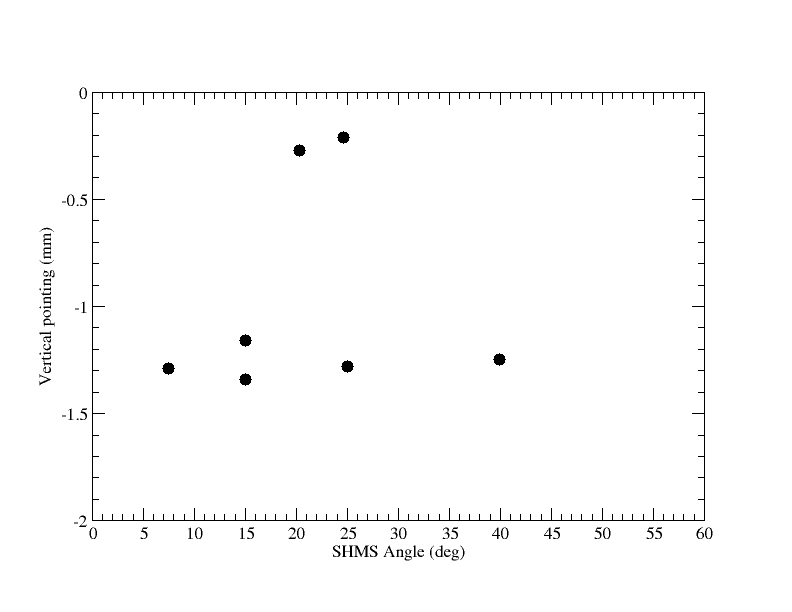
\includegraphics[width=0.8\columnwidth]{shms_vertical_pointing.png}
			\end{center}
			\caption{SHMS vertical pointing versus SHMS angle.  }
			\label{fig:shms_vert_pointing}
		\end{figure}
		
		
			\end{document}
